\documentclass{article}
\usepackage{graphicx}

\title{High-Performance Concurrent Sorted Vector Analysis}
\author{ByeongKyu Park}
\date{\today}

\begin{document}

\maketitle

\section{Introduction}

This paper details the development and performance analysis of a high-performance concurrent sorted vector, focusing on its ability to efficiently handle concurrent write and read operations. The implementation leverages modern C++ features to achieve significant performance improvements, particularly in real-time data processing applications.

\section{Performance Insights}

\subsection{Quick Sort Performance}

The parallel Quick Sort algorithm demonstrates substantial speed improvements over the traditional `std::sort` method. The performance evaluation was conducted on a system with 16 logical cores, sorting an array of 100 `Ratio` objects.

\begin{figure}[h]
\centering
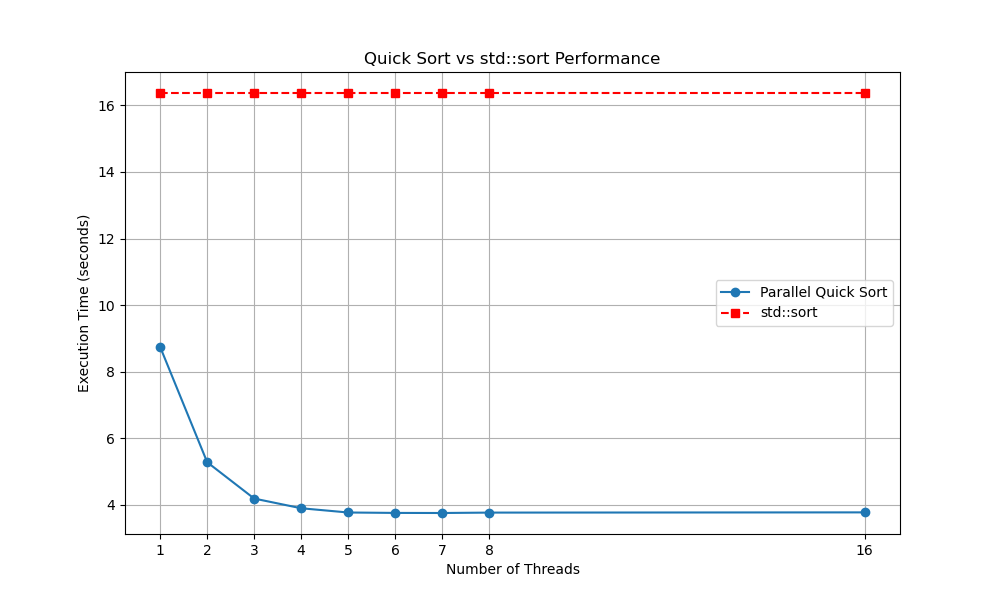
\includegraphics[width=0.8\textwidth]{QuickSortPerformanceComparison.png}
\caption{Comparison of Parallel Quick Sort and std::sort execution times.}
\label{fig:quicksort}
\end{figure}

\subsection{Concurrent Read/Write Performance}

The concurrent read/write performance was tested under varying numbers of writing threads while continuously reading from the container, showcasing the sorted vector's capability to manage high-volume concurrent modifications efficiently.

\begin{figure}[h]
\centering
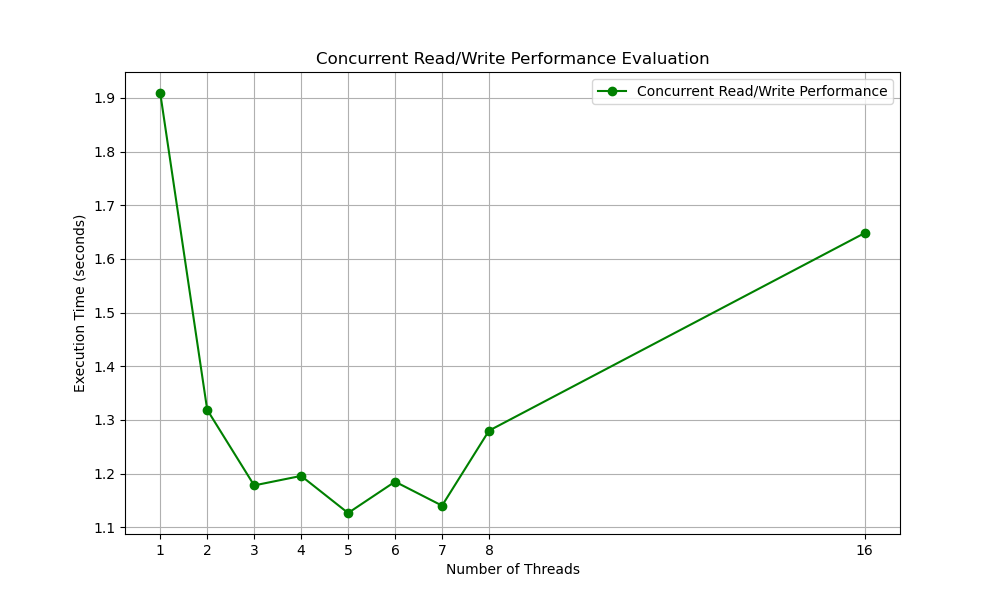
\includegraphics[width=0.8\textwidth]{ConcurrentReadWritePerformanceEvaluation.png}
\caption{Execution times for concurrent read/write operations with varying numbers of writer threads.}
\label{fig:concurrentRW}
\end{figure}

\section{Implementation Highlights}

The implementation employs a sophisticated memory management system, thread safety measures through atomic operations, and a "bag of tasks" approach for the parallel Quick Sort algorithm to distribute work among threads efficiently.

\section{The Role of the Ratio Class}

The `Ratio` class, with built-in delay for comparison operations, serves a crucial role in evaluating the time complexity and performance under simulated computational load. This approach ensures the benchmarks accurately reflect the vector's capabilities in handling complex operations.

\section{Conclusion}

The developed concurrent sorted vector represents a significant advancement in concurrent computing, offering a solution that not only excels in performance but also in efficiency and reliability for applications requiring real-time data processing.

\end{document}
